\chapter{Fundamentação Teórica}

Nesse capítulo é feita a fundamentação dos principais assuntos presentes nesse
trabalho: a heurística construtiva, as metaheurísticas e a programação
linear. Nas seções seguintes são descritas os aspectos teóricos e os
principais métodos relacionados a esse trabalho.

\section{Heurísticas Construtivas}
As técnicas de resolução heurísticas se utilizam de processos intuitivos com a
finalidade de obter uma boa solução, a um custo computacional aceitável, ou
seja não garante a otimalidade de um problema. O objetivo é obter em um tempo
reduzido uma solução tão próxima quanto possível do ótimo global.
		
Uma heurística é dita construtiva quando a construção da solução se dá elemento
por elemento. A forma de escolha dos elementos variam de acordo com a
estratégia e a função de avaliação adotada, essa escolha deve levar em
consideração o benefício da inserção de cada elemento para a solução final,
escolhendo sempre o \emph{melhor} elemento em cada passo.
		
O Algoritmo \ref{alg:heurconsgulosa} mostra o pseudocódigo para a construção de
uma solução inicial para um problema de otimização que utiliza uma função
gulosa \emph{g(.)}. Nesta figura, \emph{$t_{melhor}$} indica o membro do
conjunto de elementos candidatos com o valor mais favorável da função de
avaliação \emph{g}, isto é, aquele que possui o menor valor de \emph{g} no caso
de o problema ser de minimização ou o maior valor de \emph{g} no caso de o
problema ser de maximização.


\begin{figure}[h]
\caption{Pseudocódigo da heurística de construção gulosa de uma solução
inicial. \newline \mbox{Fonte:
\cite{notasmarcone}} }\label{alg:heurconsgulosa}
\begin{programma}
\ALGORITHM{$ConstruçãoGulosa(g(.), s$)}
\STATE s \GETS $\emptyset$;
\STATE Inicialize o conjunto $C$ de candidatos;
\WHILE{$C \neq \emptyset$}
\STATE $g(t_{melhor}) = melhor\{g(t) \mid t \in C\}$;
\STATE $s \GETS s \cup \{t_{melhor}\}$;
\STATE Atualize o conjunto $C$ de elementos candidatos;
\ENDWHILE
\STATE\RETURN $s$;
\ENDALGORITHM
\end{programma}
\end{figure}		
		

Uma outra forma de obter uma solução inicial é escolhendo os elementos
candidatos aleatoriamente. Isto é, a cada passo, o elemento a ser inserido na
solução é aleatoriamente selecionado dentre o conjunto de elementos candidatos
ainda não selecionados. A grande vantagem desta metodologia reside na
simplicidade de implementação. Segundo testes empíricos , a desvantagem é a
baixa qualidade, em média, da solução final. Essa técnica é recomendada quando
a característica do problema torna mais fácil o refinamento do que a construção
de uma solução \cite{notasmarcone}.

O Algoritmo \ref{alg:heurconsaleatoria} mostra o pseudocódigo para a construção
de uma solução inicial aleatória para um problema de otimização.

\begin{figure}[h]
\caption{Pseudocódigo da heurística de construção aleatória de uma
solução inicial. \newline \mbox{Fonte:
\cite{notasmarcone}}}\label{alg:heurconsaleatoria}
\begin{programma}
\ALGORITHM{$ConstruçãoAleatória(g(.), s$)}
\STATE s \GETS $\emptyset$;
\STATE Inicialize o conjunto $C$ de candidatos;
\WHILE{$C \neq \emptyset$}
\STATE Escolha aleatoriamente $t_{escolhido} \in C$;
\STATE $s \GETS s \cup \{t_{escolhido}\}$;
\STATE Atualize o conjunto $C$ de elementos candidatos;
\ENDWHILE
\STATE\RETURN $s$;
\ENDALGORITHM
\end{programma}
\end{figure}

Para melhores resultados essa etapa deve ser seguida de um refinamento, pois a
solução, quando gerada aleatoriamente, não costuma ser de boa qualidade.

\section{Metaheurística}

A utilização de métodos exatos para a resolução de problemas reais envolvendo
otimização combinatória é restrito. Isso acontece pois com o aumento das
instâncias envolvidas, o número de soluções possíveis cresce exponencialmente,
fazendo com que as operações necessárias para a sua resolução não possa feita
com os computadores atuais em tempo viável.

Para contornar essa limitação e obter soluções para esses tipos de problemas,
os pesquisadores desenvolveram técnicas que são capazes de guiar o procedimento
de busca e assim encontrar boas soluções \cite{maritan2009}. Esses algoritmos,
denominados heurísticas, encontram essas soluções utilizando pouco recursos
computacionais, porém não garantem a solução ótima do problema \cite{dias2006}.
Na prática, geralmente, uma boa solução é suficiente, já que a tomada de
decisão tem que acontecer em um curto espaço de tempo.

As metaheurísticas são aplicadas a uma maior gama de problemas e surgiu para
suprir algumas deficiências das heurísticas. Para contornar essas deficiências,
foram desenvolvidas técnicas mais generalistas que foram denominadas de
metaheurísticas. As metaheurísticas podem ser definidas como sendo um método
heurístico para resolver de forma genérica problemas de otimização com a
capacidade de escapar de ótimos locais. A idéia utilizada, normalmente, é
obtida de algum evento natural como sistemas biológicos, da física, da
inteligência artificial entre outros.

As metaheurísticas podem explorar o espaço de soluções basicamente de duas
formas: as metaheurísticas de busca local e as metaheurísticas de busca
populacional. Nas metaheurísticas de busca local, o procedimento de busca
utiliza uma solução como ponto de partida em cada iteração. As metaheurísticas
GRASP, arrefecimento simulado (\textit{Simulated Annealing}), busca tabu e ILS
podem ser citadas como exemplos de metaheurísticas ponto-a-ponto. Nas metaheurísticas de
busca populacionais, soluções de boa qualidade são combinadas com o intuito de
produzir soluções melhores. Podemos citar como exemplo de métodos
populacionais, os algoritmos genéticos, colônia de formigas (\textit{Ant Colony
System}), núvem de particulas (\textit{Particle Swarm Optimization}) e etc
\cite{maritan2009}.

Nesse trabalho foram utilizados as metaheurísticas de busca local GRASP e ILS
de forma híbrida. As próximas seções descrevem essas metaheurísticas.

\subsection{GRASP}

Essa seção descreve a metaheurística GRASP (\textit{Greedy Randomized Adaptive
Search Procedure} - Procedimento de busca adaptativa gulosa e randômica), que
foi proposto por \cite{resende1995}, e cujos conceitos serão
utilizados na metodologia proposta para resolução do PCTA. A metaheurística
GRASP é um método iterativo do tipo \textit{multi-start} formado por duas
fases: uma fase de construção de uma solução e outra de busca local. A fase de
construção objetiva gerar uma solução viável para o problema proposto. E a fase
de busca local na qual se pesquisa  um ótimo local na vizinhança da solução
construída. A melhor solução encontrada, ao longo de todas as
iterações GRASP realizadas, é retornada.

O pseudo-código descrito no Algoritmo \ref{alg:grasp} ilustra um procedimento
GRASP para um problema de minimização. Na linha 1 o custo da função objetivo da
melhor solução encontrada é inicializada com $\infty$(infinito). A linha 2
repete o procedimento de construção e refinamento $GRASPMax$ vezes, por causa dessa
etapa que o GRASP é considerado \textit{multi-start}.

Na linha 3 e 4 são feitas respectivamente a construção e a busca local que são
representadas nos Algoritmos \ref{alg:graspcons} e \ref{alg:grasplocal} e serão
detalhadas mais adiante.

Nas linhas 5 à 8, se a solução obtida na busca local for melhor que a melhor
solução obtida até o momento ($f(s) < f{*}$) então são atualizadas
respectivamente a solução e o custo relativo a função objetivo da melhor
solução corrente. A linha 9 encerra as iterações do GRASP e a linha 10 retorna a
melhor solução obtida na execução do algoritmo.

\begin{figure}[h]
\caption{Pseudocódigo do procedimento GRASP. \newline \mbox{Fonte:
\cite{resende1995}}}\label{alg:grasp}
\begin{programma}
\ALGORITHM{GRASP($f(.), g(.), N(.), GRASPMax, s$)}
\STATE f{*} \GETS $\infty$;
\FOR{$1, 2, ..., GRASPMax$}
\STATE Construção($g(.), \alpha, s$);
\STATE BuscaLocal($f(.),N(.),s$);
\IF{$f(s) < f{*}$}
\STATE $s{*} \GETS s$;
\STATE $f{*} \GETS f(s)$;
\ENDIF
\ENDFOR
\STATE\RETURN $s{*}$;
\ENDALGORITHM
\end{programma}
\end{figure}

Na fase de construção uma solução é iterativamente construída, elemento por
elemento. A parte gulosa da função visa gerar uma solução factível. O
componente aleatório é incluído para explorar regiões diversas do espaço de
soluções e é uma das chaves da efetividade do GRASP.

A fase de construção do GRASP é baseada na construção de uma lista restrita de
candidatos (LCR). Essa lista contem os melhores candidatos que podem ser
adicionados a solução em um dado momento, a quantidade de elementos dessa lista
é regulada pelo $\alpha$ que é um dos parâmetros do GRASP. O $\alpha$ é
definido como sendo o nível de aleatoriedade da solução.

\begin{figure}[h]
\caption{Pseudocódigo do procedimento de construção do GRASP para um problema
de minimização. \newline \mbox{Fonte:
\cite{resende1995}}}\label{alg:graspcons}
\begin{programma}
\ALGORITHM{$Construção(g(.), \alpha,s$)}
\STATE s \GETS $\emptyset$;
\STATE Inicialize o conjunto $C$ de candidatos;
\WHILE{$C \neq \emptyset$}
\STATE $g(t_{min}) \GETS min\{g(t) \mid t \in C\}$;
\STATE $g(t_{max}) \GETS max\{g(t) \mid t \in C\}$;
\STATE $LCR \GETS \{t \in C \mid g(t) \leq g(t_{min}) + \alpha(g(t_{max}) - g(t_{min}))\}$;
\STATE Selecione aleatoriamente um elemento $t \in LCR$;
\STATE $s \GETS s \cup \{t\}$;
\STATE Atualize conjunto de candidatos;
\ENDWHILE
\STATE\RETURN $s$;
\ENDALGORITHM
\end{programma}
\end{figure}

Em cada iteração são selecionados todos os elementos que podem ser
inseridos na solução e então é formada uma lista de candidatos que é ordenada
segundo algum critério pré-determinado, no caso de um problema de
minimização a lista normalmente é ordenada de acordo com o acréscimo na função
objetivo que esse elemento acarretaria se fosse escolhido. A
heurística é dita adaptativa porque os benefícios associados com a escolha de
cada elemento são atualizados em cada iteração da fase de construção para
refletir as mudanças oriundas da seleção do elemento anterior. A componente
probabilística do procedimento reside no fato de que cada elemento é
selecionado de forma aleatória a partir de um subconjunto restrito formado
pelos melhores elementos que compõem a lista de candidatos. Este subconjunto
recebe o nome de lista de candidatos restrita (LCR). Esta técnica de escolha
permite que diferentes soluções sejam geradas em cada iteração GRASP
\cite{notasmarcone}. O valor do grau de aleatoriedade $\alpha$ se encontra
entre [0,1].

Um valor de $\alpha = 0$ faz com que o algoritmo gere soluções puramente
gulosas enquanto a escolha de um $\alpha = 1$ faz com que o algoritmo gere
soluções puramente aleatórias.
 
A construção do GRASP difere do Algoritmo \ref{alg:heurconsgulosa} por causa
das linhas 4 à 7. A linha 4 obtém o valor mínimo que será acrescentado a
solução final, dentre os candidatos possíveis e a linha 5 obtém o valor máximo.
A linha 6 forma a LCR com os elementos que tiverem o valor entre $g(t_{min}) +
\alpha(g(t_{max}) - g(t_{min}))$. Por fim a linha 7 seleciona aleatoriamente um
elemento da LCR.

Com isso a quantidade de soluções possíveis é ampliada porém somente soluções
promissoras são geradas.

As soluções geradas pela fase de construção do GRASP normalmente não são
localmente ótimas com relação à definição de vizinhança adotada. Surge então a
necessidade de complementar o método com a adição de uma busca local, que tem
o objetivo de melhorar a solução construída na fase de construção. O Algoritmo
\ref{alg:grasplocal} descreve um procedimento básico de busca local relativo a
uma vizinhança $N(.)$ de $s$ para um problema de minimização. A qualidade da
construção gerada causa um impacto direto na busca local, uma vez que essa
solução inicial podem constituir pontos de partidas promissores para a busca
local, permitindo assim agilizá-los.
 
\begin{figure}[h]
\caption{Pseudocódigo do procedimento de busca local do GRASP. \newline
\mbox{Fonte:
\cite{resende1995}}}\label{alg:grasplocal}
\begin{programma}
\ALGORITHM{BuscaLocal($f(.), N(.), s$)}
\STATE $V \GETS \{s{'} \in N(s) \mid f(s{'}) < f(s)\}$;
\WHILE{$\mid V \mid > 0$}
\STATE Selecione $s{'}$ de $V$;
\STATE $s \GETS s{'}$;
\STATE $V \GETS \{s{'} \in N(s) \mid f(s{'}) < f(s)\}$;
\ENDWHILE
\STATE\RETURN $s$;
\ENDALGORITHM
\end{programma}
\end{figure}

O algoritmo de busca local define no passo 1 e 5 o conjunto de vizinhos da
solução $s{'}$ que melhoram o valor de sua função objetivo. Do passo 2 à 6 a
solução corrente é atualizada enquanto houver uma solução melhor na vizinhança.

O GRASP apresenta basicamente o parâmetro $\alpha$ que pode ser ajustado.
Valores de $\alpha$ que levem a uma LCR com tamanho bastante limitado implicam
soluções próximas as da solução gulosa, obtidas com um baixo esforço
computacional, provocamdo assim uma baixa variedade de soluções construídas, que
normalmente não é interessante para a busca local já que as soluções geradas
são muito próximas. Por outro lado a escolha de valores de $\alpha$ muito
elevado implica na geração de uma grande diversidade de soluções mas, por
outro lado, muitas das soluções construídas são de baixa qualidade.

Procedimentos GRASP mais sofisticados levam em consideração a mudança do valor
de $\alpha$ ao longo das iterações de acordo com os resultados obtidos em
iterações anteriores. Estudos feitos em \cite{prais2000} indicam que essa
adaptação do valor de $\alpha$ produz soluções melhores do que aquelas obtidas
considerando-o fixo.

\subsection{ILS}

Essa seção descreve a metaheurística ILS (Iterated Local Search - Busca Local
Iterativa) que se baseia na idéia de que um procedimento de busca local
consegue melhores resultados a medida que a solução base é variada.
Esses locais diferentes são obtidos a partir de pertubações em cima da solução
ótima local corrente.

O Algoritmo \ref{alg:ils} ilustra o pseudo-código do ILS. Nele pode-se perceber
a necessidade da definição de quatro procedimentos: (a) $GeraSoluçãoInicial()$
que obtém o ponto de partida $s_{0}$ para o problema; $BuscaLocal(s)$, que
retorna o mínimo local da solução $s$, tendo como base as estruturas de
vizinhança definidas; (c) $Pertubação(histórico, s)$, que altera a solução $s$
para outra solução, e se utiliza do histórico para evitar repetir soluções bem
como para inferir o grau de pertubação necessário para escapar do mínimo local;
E o (d) $CritérioDeAceitação(s, s{''}, histórico)$, que decide em qual solução
a próxima pertubação será aplicada.

\begin{figure}[h]
\caption{Pseudocódigo do procedimento Iterated Local Search. \newline
\mbox{Fonte:
\cite{notasmarcone}}}\label{alg:ils}
\begin{programma}
\ALGORITHM{ILS}
\STATE $s_{0}$ \GETS GeraSoluçãoInicial;
\STATE $s$ \GETS BuscaLocal($s_{0}$);
\WHILE{os critérios de parada não estiverem satisfeito}
\STATE $s{'}$ \GETS Pertubação($histórico, s$);
\STATE $s{''}$ \GETS BuscaLocal($s{'}$);
\STATE $s$ \GETS CritérioAceitação($s, s{''}, histórico$);
\ENDWHILE
\STATE\RETURN $s$;
\ENDALGORITHM
\end{programma}
\end{figure}

O ILS é dependente da escolha do método de busca local, das pertubações e do critério de aceitação. Normalmente um método de descida é utilizado, mas também é possível aplicar algoritmos mais sofisticados como Busca Tabu ou outras metaheurísticas.

A intensidade da perturbação deve ser forte o suficiente para permitir escapar do ótimo
local corrente e permitir explorar diferentes regiões. Ao mesmo tempo, ela precisa ser fraca
o suficiente para guardar características do ótimo local corrente \cite{notasmarcone}.

Um aspecto importante do critério de aceitação e da pertubação é que eles induzem aos procedimentos de intensificação e diversificação. A intensificação consiste em procurar melhores soluções nas área de busca corrente, isso acontece reduzindo a força da pertubação que faz com que as novas soluções de partida se encontrem nas proximidades da anterior. A diversificação acontece com a aplicação de grandes pertubações.

\begin{figure}[ht]
	\caption{Representação esquemática do funcionamento do ILS. \newline
	\mbox{Fonte:
	\cite{notasmarcone}}}
	\label{img:ilsfuncionamento}
	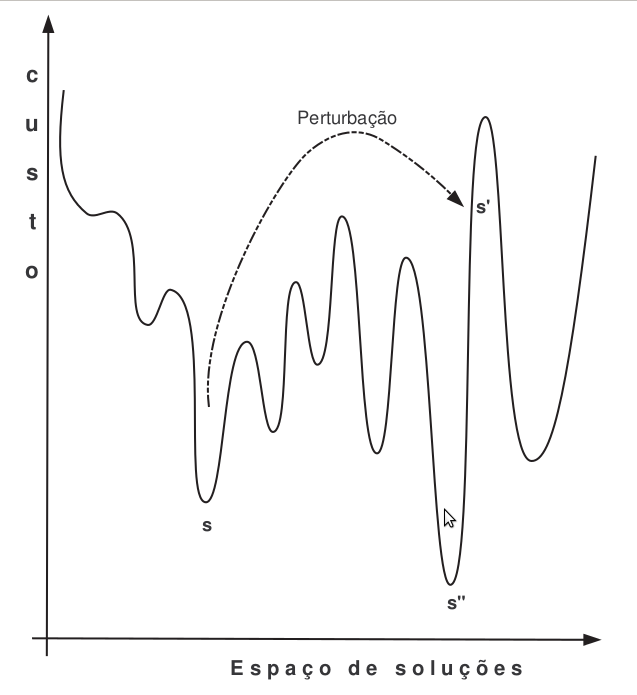
\includegraphics[scale=0.3]{./img/ilsfuncionamento.png}
\end{figure}

A Figura \ref{img:ilsfuncionamento} demonstra o funcionamento do método ILS em um problema de minimização. Dado um ótimo local $s$, é realizada uma pertubação que lhe direciona para $s{'}$. Depois da aplicação da busca local, o novo mínimo $s{''}$, melhor que a anterior, é encontrada. Ou seja $f(s{''}) < f(s)$.

Uma exemplo de pertubação seria a aplicação sucessiva de estruturas de vizinhança a solução corrente.

\section{Programação Linear}

A programação linear é provavelmente a mais conhecida e utilizada técnica de
otimização em todo o mundo e geralmente é utilizada para tomada de
decisões gerenciais sobre a alocação de recursos para produção. Os custos dos recursos e
as receitas geradas pelos produtos são usados para determinar a melhor solução.
Qualquer problema que possa ser formulado com variáveis de decisão reais, tendo
uma função objetivo linear, e funções de restrição lineares, em princípio pode
ser solucionado através da programação linear. Tais programas originariamente
utilizavam o método \textit{Simplex}, porém, recentemente, métodos de
"\textit{pontos interiores}" se mostraram mais eficientes.

Embora a programação linear seja muito eficiente para a resolução de problemas
lineares, sua aplicação a problemas que apresentem objetivos ou restrições
não-lineares tem levado a problemas e falhas de modelagem. Em alguns casos,
funções não-lineares podem ser aproximadas por algumas funções lineares
conjugadas, e a programação linear ainda pode ser utilizada. Contudo, isso leva
a uma representação ineficiente do problema, podendo causar matrizes de decisão
explosivamente grandes que demandam um tempo excessivo para resolução. Esta é
uma dificuldade comum em problemas que envolvem, por exemplo,
"\textit{scheduling}" e "\textit{sequenciamento}" de processos como é o caso do
PCTA.

De forma equivalente, outros tipos de variáveis não podem ser tratadas
diretamente com o uso de programação linear. Programação inteira usa
programação linear para resolver problemas sobre variáveis inteiras, mas ainda
com funções objetivo e restrições puramente lineares. As variáveis inteiras são
representadas como variáveis reais no algoritmo de resolução do problema. Então
um processo repetitivo é usado para "delimitar" o valor destas variáveis em
valores inteiros, através da adição de restrições e reprocessamento da solução.
Esse método, conhecido como \textit{"branch \& bound"}, finaliza quando todas
as variáveis assumem valores inteiros. Quando o número de variáveis inteiras é
pequeno, a programação inteira soluciona o problema rapidamente. Infelizmente
esse procedimento pode consumir muito tempo com um número grande de variáveis
inteiras, podendo, em alguns casos, necessitar de milhões de iterações para
serem resolvidos.
 	
Essa técnica foi muito utilizada na segunda guerra mundial para otimizar as
perdas inimigas e reduzir o custo das operações e também é utilizado no
planejamento de algumas empresas.

